In dem Abschnitt wird der Aufbau der inneren Logik der Application beschrieben. 
Für die Anwendungslogik ist ein Teil nach \textbf{SRP} (siehe Kapitel \ref{kap:SRP}) notwendig. 
Der Teil heißt \textbf{UseCase}.
Damit beim Geschehen eines Ereignisses alle \textbf{UseCases} informiert werden, 
wird ein weiterer Teil notwendig, der das Ereignis den richtigen \textbf{UseCases} zuordnet.  
Der Teil heißt \textbf{Dispatcher}.
Das Weiterleiten des Ereignisses an \textbf{Dispatcher} und das Kontrollieren von \textbf{Port} und \textbf{Adapter} wird 
vom \textbf{Controller} übernommen.

Jedes \textbf{UseCase} erledigt mehrere aufeinander folgende Aufgaben, die andere \textbf{Controller} benutzen.
Es ist vom Vorteil, andere \textbf{Controller} nicht direkt aufzurufen. 
Es kann passieren, dass es gewünscht wird gleiche Funktionalität für alle solche Aufrufe hinzuzufügen, z.B:
\begin{itemize}
    \item der Anfang und das Ende in Logs aufzeichnen.
    \item Nach einer bestimmten Zeit gestoppt werden.
\end{itemize}
Das heißt es wird um jede Methode eine ``Hülle'' gebraucht. Diese Hülle heißt \textbf{Interactor}.

Wenn alles zusammengeführt wird, entsteht folgendes Objektendiamm:

\begin{figure}[H]
    \centering
    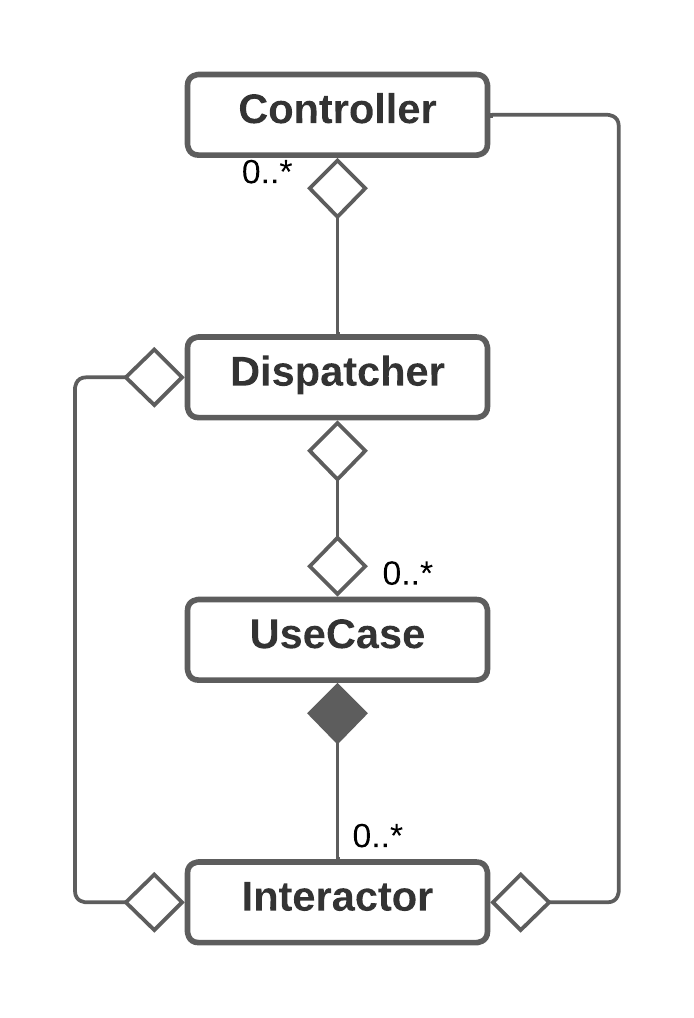
\includegraphics[width=6.5cm]{./images/Controller-Dispatcher-UseCase-Interactor.png}
     \caption[Objektendiagramm Controller-Dispatcher-UseCase-Interactor]{Objektendiagramm Controller-Dispatcher-UseCase-Interactor}
     \label{fig:CDCDUI}
\end{figure}
